%\FILE{usecase/earthquake.tex}
\subsection{Use Case: Earthquake Prediction Benchmarks}


Earthquake prediction of their occurrence and likely-hood is a complex problem. 
It is difficult because the details of
the underground plates and the friction laws between them are not
known and furthermore the earthquake causes phase transitions between
plates which makes for unpredictable movement in addition to 
predicting earthquake energy wave movements. 
Since both of these problems
are so complex with many hidden variables and the equations governing
the phenomenon are unknown or incomplete, deep learning can be use to
learn the various hidden patterns in the data which the model can then
use to forecast earthquakes into the future. \cite{fox2021earthquake}
However the application of models and hyper-parameter sets is an open challenge requiring a large amount of computational power and the investigation of several promising models.

As part of this effort a benchmark activity has been started within the MLCommons Science working Group \cite{?}. The usecase deriving from this effort motivates our efforts. Figure \ref{}fig:eq-general} shows the architecture ouf our current efforts which can be generalized to be applicable for many scientific analysis problems. More details about this application can be found at \cite{??} and \cite{??}.


\begin{figure}[htb]
\centering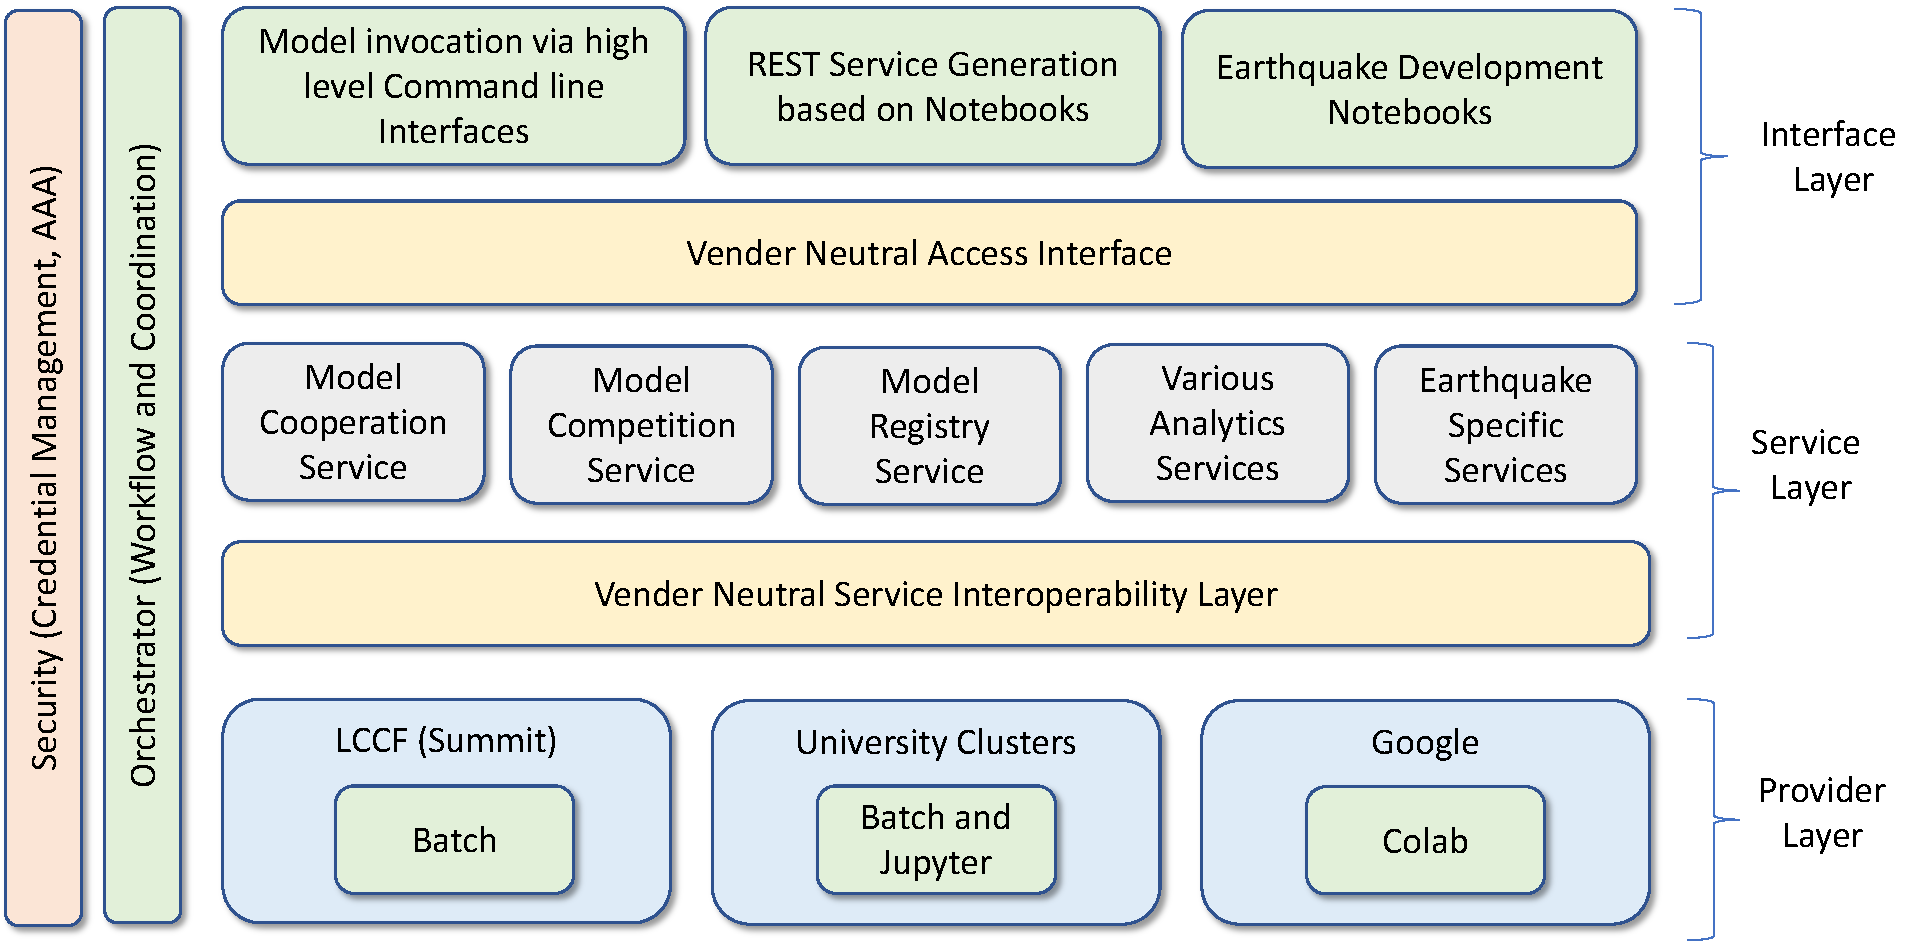
\includegraphics[width=1.0\columnwidth]{images/nist-eq-arch.pdf}
\caption{General view of Earthquake Prediction Benchmark system}
\label{fig:eq-general}
\end{figure}

This use case has the implicit requirements needing the following
aspects to be addressed by the framework we develop.

\begin{enumerate}

\item{\bf AS vendor neutral cloud and computer service integration.}

  \begin{enumerate}
  
  \item {\bf AS in cloud.} The analysis of this use case requires a significant amount of computing time as well as specialized hardware such as the utilization of GPUs. It is beneficial that the analystics services developed can run on hybrid clouds to leverage best availability and cost. Development can be supported by on-premisse resources. 
  
  \item {\bf AS in LCCF.} The availability of large HPC resources if of advantage as the calculation and hardware needs for this problem exceed those of a desktop and can benefit from running many of the models in parallel to select the best once producing a minimal scientific accuracy measurement.
  
  \item {\bf AS in microservices.} Although Microservises can be used in this effort it has not been much applied due to the greater need of accessing HPC resources.
  
  \end{enumerate}

\item{\bf AS architecture.}

  \begin{enumerate}
  
  \item{\bf AS vendor neutral interfaces.} Vendor neutral interfaces are beneficial as it would allow analytics services to be integrated in a plug-in fashion.
  
  \item{\bf AS REST.} REST services would be beneficial as the highly specialized analytics services and resources can be accessed through language and implementation neutral interfaces. This would allows the access of services by non experts, but also the integration of services that are developed by communities.

  \item{\bf AS layers such as interface, service layer, and provider layer.} As The interface layers provide the necessary abstractions to benefit from efforts across implementers specializing on various layers such as scientist, interface designers, cloud providers, and HPC providers. 

\end{enumerate}

\item{\bf AS workflow.}

  \begin{enumerate}
  
  \item{\bf AS catalog and registry.} It is beneficial to register the 
  various models and their inputs and outputs as well as performance needs and results. This way components can be chosen based on the implicit analytics performance characteristics. For example, the model of an earthquake near a volcano could be very different from a model close to the movement of a tectonic plate.

  \item{\bf AS cooperation.} The need of cooperating services and models can enhance the accuracy of the resulting new model calculation. 
  
  \item{\bf AS competition.} The integration of models found in the future and a dynamic reanalysis of the analytics functions performed earlier in case a better model is found.
 
  \item{\bf AS orchestrator.} API-based workflow definition, and orchestration capabilities are required for the coordinating the complex environments and analytics functions.
  
  \end{enumerate}


\item{\bf AS calculation.}

  \begin{enumerate}
  
  \item{\bf AS with DL.} Deep Learning is leveraged due to the complexity of the problem and the inaccessibility of details of the earth mantel.
  
  \item{\bf AS data analytics.} Data analytics is leveraged for generating the forecasts on a spatial and time dependent level.
  
  \end{enumerate}

\item{\bf AS security.} AS Security is used to control access to the various resources. As the research is carried out in an Open Source community other security issue are of little concern. 

\item{Data needs}  The data needs can become very large if real time sensors are integrated. However, smaller data sets are available and are currently used by this application to analyze Earth quakes in California from 1950 till today.
  

\end{enumerate}


\TODO{do we need to add a section dataneeds for analytics}

\TODO{we have more data than we can handle, some analytics is been done at the edge}